\documentclass[../main.tex]{subfiles}
\begin{document}
Sorting is the most basic building block for many other algorithms and is often considered as the very first step that eases and reduces the original problems to easier ones. 
\section{Introduction}
\paragraph{Sorting} In computer science, a \textit{sorting algorithm} is designed to rearrange items of a given array in a certain order based on each item's \textit{key}. The most frequently used orders are \textit{numerical order} and \textit{lexicographical order}. For example, given an array of size $n$, sort items in increasing order of its numerical values:
\begin{lstlisting}[numbers=none]
Array = [9, 10, 2, 8, 9, 3, 7]
sorted = [2, 3, 7, 8, 9, 9, 10]
\end{lstlisting}
\paragraph{Selection} \textit{Selection algorithm} is used to  find the k-th smallest number  in a given array; such a number is called the k-th \textit{order statistic}. For example, given the above array, find the 3-th smallest number.
\begin{lstlisting}[numbers=none]
Array = [9, 10, 2, 8, 9, 3, 7], k = 3
Result: 7
\end{lstlisting}
Sorting and Selection often go hand in hand; either we first execute sorting and then select the desired order through indexing or we derive a selection algorithm from a corresponding sorting algorithm. Due to such relation, this chapter is mainly about introducing sorting algorithms and occasionally we introduce their corresponding selection algorithms by the side. 

\paragraph{Lexicographical Order} For a list of strings, sorting them will make them in lexicographical order. The order is decided by a comparison function, which compares corresponding characters of the two strings from left to right. In the process,  the first  pair of characters that differ from each other  determines the ordering: the string that has smaller alphabet from the pair is smaller than the other string. 

Characters are compared using the Unicode character set. All uppercase letters come before lower case letters. If two letters are the same case, then alphabetic order is used to compare them. For example:
\begin{lstlisting}[numbers=none]
'ab' < 'bc' (differs at i = 0)
'abc' < 'abd' (differs at i = 2)
\end{lstlisting}
Special cases appears when two strings are of different length and the shorter one $s$ is a prefix of the the longer one $t$, then it is considered that $s < t$. For example: 
\begin{lstlisting}[numbers=none]
'ab' < 'abab' ('ab' is a prefix of 'abab')
\end{lstlisting} 

\paragraph{How to Learn Sorting Algorithms?} We list a few terminologies that are commonly seen to describe the properties of a certain sorting algorithm:
% \paragraph{How to Learn Sorting Algorithms?}  Before we start our journey to learn each individual existing sorting algorithm, it is worthy the time to discuss some key terminologies and techniques that distinguish different kind. Therefore, along the learning process, we know what questions to answer and trying to look for answer. Knowing the behavior and performance of each kind helps us making better decision when trying to design  best solutions for real problems. 
\begin{itemize}
    \item \textbf{In-place Sorting}: In-place sorting algorithm only uses a constant number of extra spaces to assist its implementation. If a sorting algorithm is not in-place, it is called out-of-place sorting instead. 
    \item \textbf{Stable Sorting}: Stable sorting algorithm maintain the relative order of items with equal keys. For example, two different tasks that come with same priority in the priority queue should be scheduled in the relative pending ordering.
    \item \textbf{Comparison-based Sorting}: This kind of sorting technique determines the sorted order of an input array by comparing pairs of items and moving them around based on the results of comparison. And it has a lower bound of $\Omega (n\log n)$ comparison. 
\end{itemize}

\paragraph{Sorting Algorithms in Coding Interviews}  As the fundamental Sorting and selection algorithms can still be potentially met in interviews where we might be asked to implement and analyze any sorting algorithm you like. Therefore, it is necessary for us to understand the most commonly known sorting algorithms. Also, Python provides us built-in sorting algorithms to use directly and we shall mater the syntax too.

\paragraph{The Applications of Sorting} The importance of sorting techniques is decided by its multiple fields of application:
\begin{enumerate}
    \item Sorting can organize information in a human-friendly way. For example, the lexicographical order are used in dictionary and inside of library systems to help users locate wanted words or books in a quick way. 
    \item Sorting algorithms often be used as a key subroutine to other algorithms. As we have shown before, binary search, sliding window algorithms, or cyclic shifts of suffix array need the data to be in sorted order to carry on the next step. When ordering will not incur wrong solution to the problems, sorting beforehand should always be atop on our mind for sorting first might ease our problem later. 
\end{enumerate}

\paragraph{Organization} We organize the content mainly based on the worst case time complexity. Section~\ref{o_n_2_sorting} - \ref{o_n_log_n_sorting} focuses on comparison-based sorting algorithms, and Section~\ref{O_n_k_sorting}-\ref{o_n_sorting} introduce classical non-comparison-based sorting algorithms. %In addition, Section~\ref{lexcographical_order} completes the picture and show which sorting algorithms can be adapted to do lexcographical order sorting based on its distinct characters that the range of keys limited by $|\sum|$, the number of possible keys in the definition. Further, in Section~\ref{python_built_in_sort}, we introduce the built-in sort function. Know the properties and how to customize the comparison functions. To recap:
\begin{itemize}
\item Naive Sorting (Section~\ref{o_n_2_sorting}): Bubble Sort, Insertion Sort, Selection Sort;
\item Asymptotically Best Sorting (Section~\ref{o_n_log_n_sorting}) Sorting: merge sort, quick sort, and Quick Select;
\item Linear Sorting (Section~\ref{O_n_k_sorting}): Counting Sort, where $k$ is the range of the very first and last key.
\item  Python Built-in Sort (Section~\ref{python_built_in_sort}):  
\end{itemize}
% We can get $O(1)$ for an sorted data strcture. The simplest case of a selection algorithm is finding the minimum (or maximum) item by iterating through the data structure, and the hardest case is finding the median. Many selection algorithms are derived by generalizing a sorting algorithm. Naturally, sorting  can potentially be the first step of algorithms like selection or even other problems to ordering the data. Such as we can apply binary search on the sorted data structure. 

% The best-known selection algorithm is quickselect, which is related to quicksort.  Naturally sorting is  the most basic and fundamental step in problem solving and many languages have provided us built-in sorting algorithms to use directly. 

\section{Python Comparison Operators and Built-in Functions} 
\paragraph{Comparison Operators} Python offers 7 comparison operators shown in Table.~\ref{tab:comparison_operators} to compare values. It either returns \texttt{True} or \texttt{False} according to the condition. 

\begin{table}[h]
\begin{small}
\centering
\noindent\captionof{table}{Comparison operators in Python}
 \noindent \begin{tabular}{|p{0.25\columnwidth}|p{0.65\columnwidth}|}
 \hline
> & Greater than - \texttt{True} if left operand is greater than the right\\ \hline
< &	Less that - \texttt{True} if left operand is less than the right\\ \hline
== 	& Equal to - \texttt{True} if both operands are equal\\ \hline
!= &	Not equal to - \texttt{True} if operands are not equal\\ \hline
>= 	& Greater than or equal to - \texttt{True} if left operand is greater than or equal to the right\\ \hline
<= 	& Less than or equal to - True if left operand is less than or equal to the right\\ \hline
\end{tabular}
  \label{tab:comparison_operators}
  \end{small}
\end{table} 

For example, compare two numerical values:
\begin{lstlisting}[language=Python]
c1 = 2 < 3
c2 = 2.5 > 3
\end{lstlisting}
The printout is:
\begin{lstlisting}[language=Python]
(True, False)
\end{lstlisting}
Also, compare two strings follows the lexicographical orders:
\begin{lstlisting}[language=Python]
c1 = 'ab' < 'bc'
c2 = 'abc' > 'abd'
c3 = 'ab' < 'abab'
c4 = 'abc' != 'abc'
\end{lstlisting}
The printout is:
\begin{lstlisting}[language=Python]
(True, False, True, False)
\end{lstlisting}
What's more, it can compare other types of sequences such as \texttt{list} and \texttt{tuple} using lexicographical orders too:
\begin{lstlisting}[language=Python]
c1 = [1, 2, 3] < [2, 3]
c2 = (1, 2) > (1, 2, 3)
c3 = [1, 2] == [1, 2]
\end{lstlisting}
The printout is:
\begin{lstlisting}[language=Python]
(True, False, True)
\end{lstlisting}
However, mostly Python 3 does not support comparison between different types of sequence, nor does it supports comparison for \texttt{dictionary}.  For \texttt{dictionary} data structures, in default, it uses its key as the key to compare with. For example, comparison between \texttt{list} and \texttt{tuple} will raise \texttt{TypeError}:
\begin{lstlisting}[language=Python]
[1, 2, 3] < (2, 3)
\end{lstlisting}
The error is shown as:
\begin{lstlisting}[language=Python]
----> 1 [1, 2, 3] < (2, 3)
TypeError: '<' not supported between instances of 'list' and 'tuple'
\end{lstlisting}
Comparison between dictionary as follows will raise the same error:
\begin{lstlisting}[language=Python]
{1: 'a', 2:'b'} < {1: 'a', 2:'b', 3:'c'}
\end{lstlisting}
\paragraph{Comparison Functions} 
Python built-in functions \texttt{max()} and \texttt{min()} support two forms of syntax: \texttt{max(iterable, *[, key, default])} and \texttt{max(arg1, arg2, *args[, key])}. If one positional argument is provided, it should be an iterable. And then it returns the largest item in the iterable based on its key. It also accepts two or more positional arguments, and these arguments can be numerical or sequential. When there are two or more positional argument, the function returns the largest. 

For example, with one iterable and it returns \texttt{20}:
\begin{lstlisting}[language=Python]
max([4, 8, 9, 20, 3])
\end{lstlisting}
With two positional arguments --either numerical or sequential:
\begin{lstlisting}[language=Python]
m1 = max(24, 15)
m2 = max([4, 8, 9, 20, 3], [6, 2, 8])
m3 = max('abc', 'ba')
\end{lstlisting}
The printout of these results is:
\begin{lstlisting}[language=Python]
(24, [6, 2, 8], 'ba')
\end{lstlisting}
With \texttt{dictionary}:
\begin{lstlisting}[language=Python]
dict1 = {'a': 5, 'b': 8, 'c': 3}
k1 = max(dict1)
k2 = max(dict1, key=dict1.get)
k3 = max(dict1, key =lambda x: dict1[x])
\end{lstlisting}
The printout is:
\begin{lstlisting}[language=Python]
('c', 'b', 'b')
\end{lstlisting}
When the sequence is empty, we need to set an default value:
\begin{lstlisting}[language=Python]
max([], default=0)
\end{lstlisting}
\paragraph{Rich Comparison} To compare a self-defined \texttt{class}, in Python 2.X, \texttt{\_\_cmp\_\_(self, other)} special method is used to implement comparison between two objects. \texttt{\_\_cmp\_\_(self, other)} returns negative value if \texttt{self < other}, positive if \texttt{self > other}, and zero if they were equal. However, in Python 3, this \texttt{cmp} style of comparisons is dropped, and \texttt{rich comparison} is introduced, which assign a special method to each operator as shown in Table.~\ref{tab:comparison_operator_special_method}: 
\begin{table}[h]
\begin{small}
\centering
\noindent\captionof{table}{Operator and its special method}
 \noindent \begin{tabular}{|p{0.25\columnwidth}|p{0.35\columnwidth}|}
 \hline
== & \texttt{\_\_eq\_\_} \\ \hline
!= &\texttt{\_\_ne\_\_}\\ \hline
< 	& \texttt{\_\_lt\_\_}\\ \hline
<= &\texttt{\_\_le\_\_}\\ \hline
> 	& \texttt{\_\_gt\_\_}\\ \hline
>= 	& \texttt{\_\_ge\_\_}\\ \hline
\end{tabular}
  \label{tab:comparison_operator_special_method}
  \end{small}
\end{table} 
To avoid the hassle of providing all six functions, we can only implement \texttt{\_\_eq\_\_}, \texttt{\_\_ne\_\_}, and only one of the ordering operators, and use the \texttt{functools.total\_ordering()} decorator to fill in the rest. For example, write a class \texttt{Person}:
\begin{lstlisting}[language=Python]
from functools import total_ordering
@total_ordering
class Person(object):
    def __init__(self, firstname, lastname):
        self.first = firstname
        self.last = lastname

    def __eq__(self, other):
        return ((self.last, self.first) == (other.last, other.first))
        
    def __ne__(self, other):
        return not (self == other)

    def __lt__(self, other):
        return ((self.last, self.first) < (other.last, other.first))

    def __repr__(self):
        return "%s %s" % (self.first, self.last)
\end{lstlisting}
Then, we would be able to use any of the above comparison operator on our class:
\begin{lstlisting}[language=Python]
p1 = Person('Li', 'Yin')
p2 = Person('Bella', 'Smith')
p1 > p2
\end{lstlisting}
It outputs \texttt{True} because last name ``Yin'' is larger than ``Smith''.
%%%%%%%%%%%%%%%%
% Chapter: Bubble sort %
%%%%%%%%%%%%%%%%
\section{Naive Sorting}
\label{o_n_2_sorting}
As the  most naive and intuitive group of comparison-based sorting methods, this group takes $O(n^2)$ time and  usually consists of two nested for loops. In this section, we learn three different sorting algorithms ``quickly'' due to their simplicity: insertion sort, bubble sort,and selection sort.



\subsection{Insertion Sort}
Insertion sort is one of the most intuitive sorting algorithms for humans. For humans, given an array of $n$ items to process, we divide it into two regions: \textbf{sorted and unrestricted region}. Each time we take one item ``out'' of the unrestricted region  to sorted region by inserting it at a proper position. 

\begin{figure}[!ht]
    \centering
    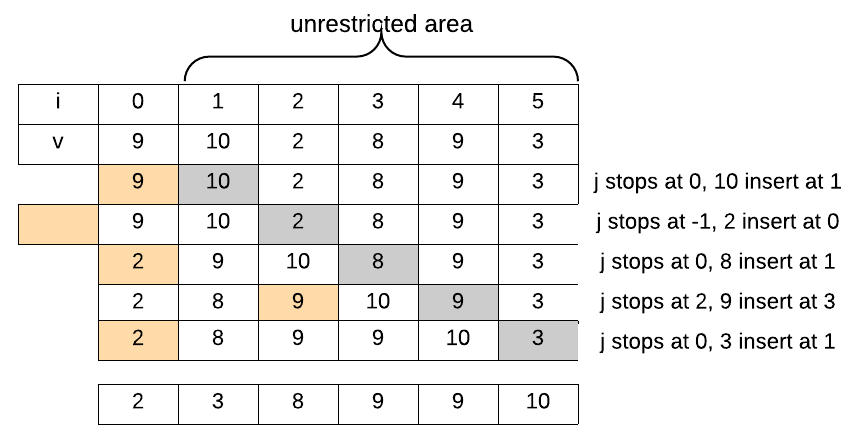
\includegraphics[width=0.9\columnwidth]{fig/insertion_sort.png}
    \caption{The whole process for insertion sort:  Gray marks the item to be processed, and yellow marks the position after which the gray item is to be inserted into the sorted region.}
    \label{fig:insertion_sort}
\end{figure}



\paragraph{In-place Insertion} The logic behind this algorithm is simple, we can do it easily by setting up another sorted array. However, here we want to focus on the in-place insertion. Given array of size $n$, we use index $0$ and $i$ to point to the start position of sorted and the unrestricted region, respectively. And $i=1$ at the beginning, indicates that the sorted region will naturely has one item. We have sorted region in $[0, i-1]$, and the unrestricted region in $[i, n-1]$. We scan item in the unrestricted region from left to right, and insert each item $a[i]$ into the sorted sublist. 

The key step is to find a proper position of $a[i]$ in the region $[0, i-1]$ to insert into. There are two different ways for iteration over unsorted region: forward and backward. We use pointer $j$ in the sorted region.
\begin{itemize}
    \item Forward: $j$ will iterate in range $[0, i-1]$. We compare $a[j]$ with $a[i]$, and stop at the first place that $a[j] > a[i]$ (to keep it stable).  All items elements $a[j:i-1]$ will be shifted backward for one position, and $a[i]$ will be placed at index $j$. Here we need $i$ times of comparison and swaps. 
    
    \item Backward: $j$ iterates in range $[i-1, 0]$. We compare $a[j]$ with $a[i]$, and stop at the first place that $a[j] <= a[i]$ (to keep it stable). In this process, we can do the shifting simultaneously: if $a[j] > a[i]$, we shift $a[j]$ with $a[j+1]$. 
\end{itemize}
In forward, the shifting process still requires us to reverse the range,
therefore the backward iteration makes better sense.

For example, given an array $a = [9, 10, 2, 8, 9, 3]$. First, 9 itself is sorted array. we demonstrate the backward iteration process. At first, 10 is compared with 9, and it stays at where it is. At the second pass, 2 is compared with 10, 9, and then it is put at the first position. The whole  whole process of this example is demonstrated in Fig.~\ref{fig:insertion_sort}. 


% If the $t$ is larger than $v$, we keep comparing the next $v$; if $t$ is smaller or equal to $v$, we insert $t$ at the place of $v$. In python using the insert() of the list data type will automatically shift items behind. Doing so will keep the sorting to be stable, that is the items with equal keys will remain its original order. However, if the $t$ is larger than all the items, then we need to remember to insert it at the end. 
% \begin{lstlisting}[numbers=none]
% If the t > v:
%     we move to the next v
% else t <= v: # we
%   insert at the position of v
% \end{lstlisting}


\paragraph{With Extra Space Implementation} The Python \texttt{list.insert()} function handles the insert and shifting at the same time. We need to pay attention when the item is larger than all items in the sorted list, we have to insert it at the end.
\begin{lstlisting}[language=Python]
def insertionSort(a):
  if not a or len(a) == 1:
    return a
  n = len(a)
  sl = [a[0]] # sorted list
  for i in range(1, n):
    for j in range(i):
      if sl[j] > a[i]:
        sl.insert(j, a[i])
        break
    if len(sl) != i + 1: # not inserted yet
      sl.insert(i, a[i])
  return sl
\end{lstlisting}
\paragraph{Backward In-place Implementation}
We use a \texttt{while} loop to handle the backward iteration: whenever the target is smaller than the item in the sorted region, we shift the item backward. When the \texttt{while} loop stops, it is either $j = -1$ or when $t >= a[j]$. 
\begin{itemize}
    \item When $j=-1$, that means we need to insert the target at the first position which should be $j+1$. 
\item When $t >= a[j]$, we need to insert the target one position behind $j$, which is $j+1$. 
\end{itemize}
The code is shown as:
\begin{lstlisting}[language=Python]
def insertionSort(a):
  if not a or len(a) == 1:
    return a
  n = len(a)
  for i in range(1, n):
    t = a[i]
    j = i - 1
    while j >= 0 and t < a[j]: 
      a[j+1] = a[j] # Move item backward
      j -= 1
    a[j+1] = t      
  return
\end{lstlisting}


% The detail is for each element that is going to be inserted, for the case of increasing order, we reversely iterate through the sorted list, if the current value is larger, then put the element in current position, otherwise, shift the larger element backward, and compare it with the element before it. The Python code is as follows:
% \begin{lstlisting}[language = Python]

% def shift(a, start, end):
%   for i in range(end, start, -1): # [i, j)
%     a[i] = a[i-1]
    
% def insertionSort(a):
%   if not a or len(a) == 1:
%     return a
%   n = len(a)
%   sl = [a[0]] # sorted list
%   for i in range(1, n): # items to be inserted into the sorted
%     for j in range(i):
%       if a[i] <= a[j]:
%         # shift all other elements [j, i-1]
%         tmp = a[i]
%         shift(a, j, i)
%         a[j] = tmp
    
%   return a
  
% def insertionSort(alist):
%   for index in range(1,len(alist)):

%      currentvalue = alist[index]
%      position = index

%      while position>0 and alist[position-1]>currentvalue:
%          alist[position] = alist[position-1] #shift the larger element back
%          position = position-1

%      alist[position] = currentvalue
% alist = [54,26,93,17,77,31,44,55,20]
% insertionSort(alist)
% print(alist)
% \end{lstlisting}

\subsection{Bubble Sort and Selection Sort}
\subsubsection{Bubble Sort}
Bubble sort compares each pair of adjacent items in an array and swaps them if they are out of order. Given an array of size $n$: in a single pass, there are $n-1$ pairs  for comparison, and at the end of the pass, one item will be put in place. 
\begin{figure}[H]
    \centering
    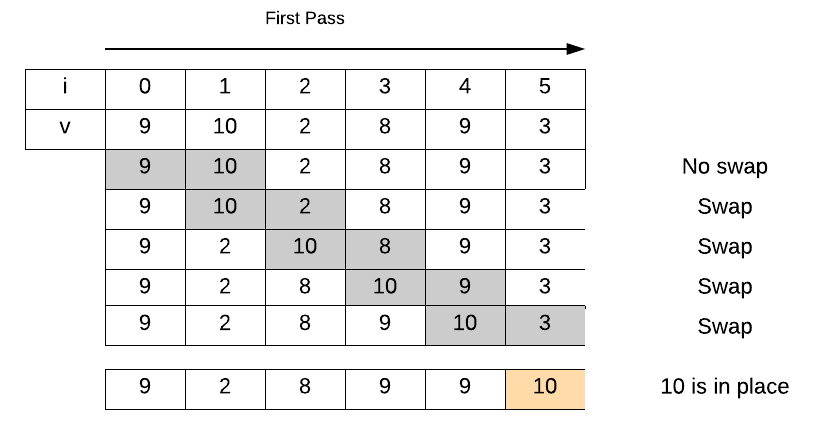
\includegraphics{fig/bubble_sort.png}
    \caption{One pass for bubble sort}
    \label{fig:bubble_sort}
\end{figure}

\paragraph{Passes}  For example, Fig.~\ref{fig:bubble_sort} shows the first pass for sorting array [9, 10, 2, 8, 9, 3]. When comparing a pair $(a_i, a_{i+1})$, if $a_i > a_{i+1}$, we swap these two items. We can clearly see after one pass, the largest item 10 is in place. For the next pass, it only compare pairs within the unrestricted window $[0, 4]$.  This is what``bubble'' means in the name: after a pass, the largest item in the unrestricted window bubble up to the end of the window and become in place. 

% \paragraph{Next Pass} Therefore, in the next pass, the last item will no longer needed to be compared. For pass $i$, it places the current $i$-th largest items in position in range of $[n-i-1, n)$.  the last $i$ items will be sorted.  We say, in the first pass, where $i=0$, the valid window is $[0, n)$, and to be generalize the valid window for $i$-th pass is $[0, n-i)$.  

\paragraph{Implementation} With the understanding of the valid window of each pass, we can implement ``bubble'' sort with two nested \texttt{for} loops in Python. The first \texttt{for} loop to enumerate the number of passes, say $i$, which is  $n-1$ in total. The second \texttt{for} loop to is to scan pairs in the unrestricted window $[0, n-i-1]$ from left to right. thus index $j$ points to the first item in the pair, making it in range of $[0, n-i-2]$.
\begin{lstlisting}[language = Python]
def bubbleSort(a):
  if not a or len(a) == 1:
    return 
  n = len(a)
  for i in range(n - 1): #n-1 passes 
    for j in range(n - i -1): 
      # Swap
      if a[j] > a[j + 1]:
        a[j], a[j + 1] = a[j + 1], a[j] 
  return
\end{lstlisting}
When the pair has equal values, we do not need to swap them. The advantage of doing so is (1) to save unnecessary swaps and (2) keep the original order of items with same keys. This makes bubble sort a \textbf{stable sort}.  Also, in the implementation no extra space is assigned either which makes bubble sort \textbf{in-place sort}.

% The most basic and most intuitive sorting algorithm is the bubble sort. The bubble sort makes multiple passes through a list. In each pass, it compare a pair of adjacent items and switch them if they are out of order. For pass $i$, it places the current $i$th largest value in position $n-i$. In essence, each item “bubbles” up to the location where it belongs. The time complexity of bubble sort is $O(n+(n-1)+(n-2)+...+1)= O(n(n-1)/2) = O(n^2)$. 

% Figure ~\ref{fig:bubble_sort} shows the first pass of a bubble sort. The shaded items are being compared to see if they are out of order. If there are n items in the list, then there are n-1 pairs of items that need to be compared on the first pass. It is important to note that once the largest value in the list is part of a pair, it will continually be moved along until the pass is complete.


\paragraph{Complexity Analysis and Optimization} In $i$-th pass, the item number in the valid window is $n-i$ with $n-i-1$ maximum of comparison and swap, and we need a total of $n-1$ passes. The total time will be $T = \sum_{i=0}^{n-i}{(n-i-1)} = n-1 + (n-2) +...+2+1 = n(n-1)/2=O(n^2)$. The above implementation runs $O(n^2)$ even if the array is sorted. We can optimize the inner \texttt{for} loop by stopping the whole program if no swap is detected in a single pass. When the input is nearly sorted, this strategy can get us $O(n)$ time complexity.

% \to sort, this makes it in-place sort. Also, it is a stable sort. paragraph{Properties} As we see in bubble sort, there is no extra space needed 
\subsubsection{Selection Sort}
\begin{figure}[!ht]
    \centering
    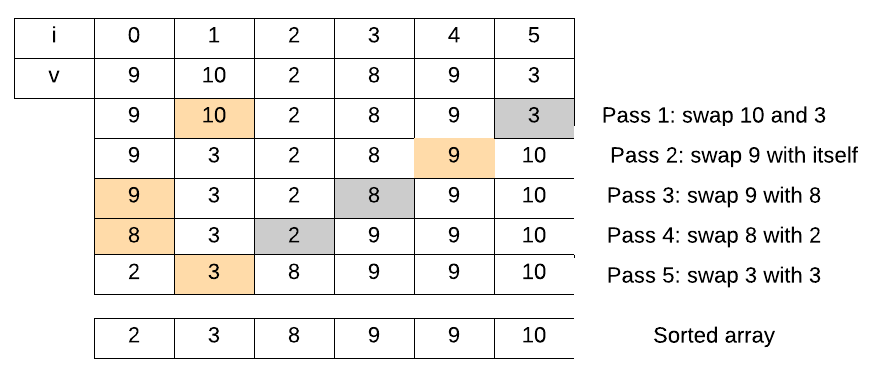
\includegraphics[width=0.98\columnwidth]{fig/selection_sort.png}
    \caption{The whole process for Selection sort}
    \label{fig:selection_sort}
\end{figure}
In the bubble sort, each pass we get the largest element in the valid window in place by a series of swapping operations. While, selection sort makes a slight optimization via searching for the largest item in the current unrestricted window and swap it directly with the last item in the  region. This avoids the constant swaps as occurred in the bubble sort. The whole sorting process for the same array is shown in Fig~\ref{fig:selection_sort}.

\paragraph{Implementation} Similar to the implementation of Bubble Sort, we have the concept of number of passes at the outer \texttt{for} loop, and the concept of unrestricted  at the inner \texttt{for} loop. We use variables \texttt{ti} and 
\texttt{li} for the position of the largest item to be and being, respectively.
\begin{lstlisting}[language = Python]
def selectSort(a):
  n = len(a)
  for i in range(n - 1): #n-1 passes 
    ti = n - 1 - i
    li = 0 # The index of the largest item
    for j in range(n - i):
      if a[j] >= a[li]:
        li = j
    # swap li and ti
    a[ti], a[li] = a[li], a[ti]
  return 
\end{lstlisting}
Like bubble sort, selection sort is \textbf{in-place}. In the comparison, we used \texttt{if a[j] >= a[li]:}, which is able to keep the relative order of equal keys. For example, in our example, there is equal key $9$. Therefore, selection sort is stable sort too.

\paragraph{Complexity Analysis} Same as of bubble sort, selection sort has a worst and average time complexity of $O(n^2)$ but more efficient when the input is not as near as sorted. 
%%%%%%%%%%%%%%%%
% Chapter: Merge Sort %
%%%%%%%%%%%%%%%%
\section{Asymptotically Best Sorting}
\label{o_n_log_n_sorting}
We have learned a few comparison-based sorting algorithms and they all have an upper bound of $n^2$ in time complexity due to the number of comparisons must be executed. Can we do better than $O(n^2)$ and how? 

\paragraph{Comparison-based Lower Bounds for Sorting} Given an input of size $n$, there are $n!$ different possible permutations on the input, indicating that our sorting algorithms must find the one and only one permutation by comparing pairs of items. So, how many times of comparison do we need to reach to the answer? Let's try the case when $n=3$, and all possible permutations using the indexes will be: $(1,2,3), (1,3,2), (3,1,2), (2,1,3), (2,3,1),(3,2,1)$. First we compare pair $(1,2)$, if $a_1 < a_2$, our candidates set is thus narrowed down to $\{(1,2,3), (1,3,2), (3,1,2)\}$. 

We draw a decision-tree, which is a full binary tree with $n!$ leaves--the $n!$ permutations, and each branch represents one decision made on the comparison result. The cost of any comparison-based algorithm is abstracted as the length of the path from the root of the decision tree to its final sorted permutation. The longest path represents the worst-case number of comparisons. 

Using $h$ to denote the height of the binary tree, and $l$ for the number of leaves. First, a binary tree will have at most $2^h$ leaves, we get $l \leq 2^h$. Second, it will have at least $n!$ leaves to represent all possible orderings, we have $l \geq n!$ . Therefore we get the lower bound time complexity for the worst case:
\begin{align}
n! &\leq l \leq 2^h \\
    2^h &\ge n!\\
    h &\ge \log(n!) \\
    h &= \Omega(n\log n)
\end{align}

In this section, we will introduce three classical sorting algorithms that has $O(n\log n)$ time complexity: Merge Sort and Quick Sort both utilize the Divide-and-conquer method, and Heap Sort uses the max/min heap data structures.
\subsection{Merge Sort}
% We have already used Merge Sort as the basic example of illustrating the Divide-and-Conquer algorithm design methodology. 
As we know there are two main steps: ``divide'' and ``merge'' in merge sort and we have already seen the illustration of the ``divide'' process in Chapter.~\ref{chapter_divide_conquer}. %and each happens at a differnt stage of the recursion function call. 

\paragraph{Divide} In the divide stage, the original problem $a[s...e]$, where $s, e$ is the start and end index of the subarray, respectively. The divide process divides its parent problem into two halves from the middle index $m = (s+e)//2$: $a[s...m]$, and $a[m+1, e]$. This recursive call keeps moving downward till the size of the subproblem becomes one when $s=e$, which is the base case for a list of size 1  is naturally sorted. The process of divide is shown in Fig.~\ref{fig:merge_sort}.

\begin{figure}[!ht]
    \centering
    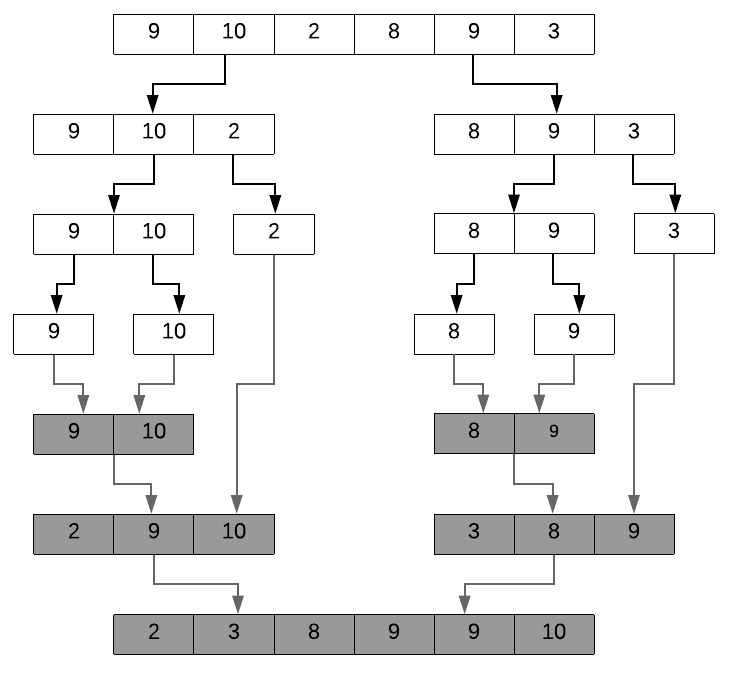
\includegraphics[width=0.9\columnwidth]{fig/merge_sort.png}
        \caption{Merge Sort: The dividing process is marked with dark arrows and the merging process is with gray arrows with the merge list marked in gray color too.}
    \label{fig:merge_sort}
\end{figure}

\paragraph{Merge} When we obtained two sorted sublists from the left and right side, the result of current subproblem is to merge the two sorted list into one. The merge process is done through two pointer method:  We assign a new list and put two pointers at the start of the two sublists, and each time we choose the smaller item to append into the new list between the items indicated by the two pointers. Once a smaller item is chosen, we move its corresponding pointer to the next item in that sublist. We continue this process  until any pointer reaches to the end. Then, the sublist where the pointer does not reach to the end yet is coped to the end of the new generated list.  The subprocess is shown in Fig.~\ref{fig:merge_sort} and its implementation  is as follows:
\begin{lstlisting}[language=Python]
def merge(l, r): 
  ans = []
  # Two pointers each points at l and r
  i = j = 0 
  n, m = len(l), len(r)

  while i < n and j < m: 
    if l[i] <= r[j]:
      ans.append(l[i])
      i += 1
    else:
      ans.append(r[j])
      j += 1
      
  ans += l[i:]
  ans += r[j:]
  return ans
\end{lstlisting}

In the code, we use $l[i] <= r[j]$ instead of $l[i] < r[j]$ is because when the left and right sublist contains items of equal keys,  we put the ones in the left first in the merged list, so that the sorting can be  \textbf{stable}. However, we used a temporary space as $O(n)$ to save the merged result a, making merge sort an  \textbf{ out-of-place} sorting algorithm.

\paragraph{Implementation} The whole implementation is straightforward. 
\begin{lstlisting}[language = Python]
def mergeSort(a, s, e):
  if s == e:
    return [a[s]]

  m = (s + e) // 2 

  l = mergeSort(a, s , m)
  r = mergeSort(a, m+1, e)
  return merge(l, r)
\end{lstlisting}
% Check out the sample code to how to prove a sorting is stable or not using tuple.  


\paragraph{Complexity Analysis} Because for each divide process we need to take $O(n)$ time to merge the two sublists back to a list, the recurrent relation of the complexity function can be deducted as follows: 
\begin{equation} \label{bt_time}
\begin{split}
T(n) & = 2T(n/2) + O(n)\\
 & = 2 * 2T(n/4) + O(n) + O(n)\\
 & = O(n\log n)
\end{split}
\end{equation}
Thus, we get $O(n\log n)$ as the upper bound for merge sort, which is asymptotically optimal within the comparison-based sorting.

\subsection{HeapSort}
\label{sorting_subsec_heapsort}
To sort the given array in increasing order, we can use min-heap. We first \texttt{heapify} the given array. To get a sorted list, we  can simply pop out items till the heap is empty. And the popped out items will be in sorted order. 

%Since the maximum item is stored at the root, we can put swap root with the last item in the list, and then we can view the heap as a smaller size of $n-1$. We observe all the subtree of the root remain max-heaps other than the new root item that might violate the max-heap property. We restore the max-heap property through sinking, and put the root item at position $n-2$, and repeat the process for n-1 times.  

% \paragraph{Implementation} Continuing use our examplary Heap class in Chapter~\ref{chapter_heap_priority_queue}, we implement heapsort member function: 
% \begin{lstlisting}[language=Python]
%     def heapsort(self, a):
%       self.heapify_sink(a)
%       n = len(a)
%       for i in range(n, 1, -1): # position to put the root node
%         self.heap[i], self.heap[1] = self.heap[1], self.heap[i] #swap root with i
%         self.size -= 1
%         self._sink(1) # sink dow the new root
%         print(self.heap)
% \end{lstlisting}
\paragraph{Implementation}
We can implement heap sort easily with  built-in module \texttt{heapq}  through the \texttt{heapify()} and \texttt{heappop()} functions :
\begin{lstlisting}[language=Python]
from heapq import heapify, heappop
def heapsort(a):
  heapify(a)
  return [heappop(a) for i in range(len(a))]
\end{lstlisting}

\paragraph{Complexity Analysis} The \texttt{heapify}  takes $O(n)$, and the later process takes $O(\log n + \log {(n-1)} +... + 0) = \log (n!)$ which has an upper bound of $O(n\log n)$. %Check out more on \url{https://www.programiz.com/dsa/heap-sort}.
%%%%%%%%%%%%%%%%
% Chapter: Quick Sort %
%%%%%%%%%%%%%%%%
\subsection{Quick Sort and Quick Select}
Like merge sort, quick sort applies divide and conquer method and is mainly implemented with recursion. Unlike merge sort, the conquering step the sorting process- \textit{partition} happens before ``dividing'' the problem into subproblems through recursive calls.  

\paragraph{Partition and Pivot} In the partition, quick sort chooses a \textit{pivot} item from the subarray, either randomly or intentionally. Given a subarray of $A[s, e]$, the pivot can either be located  at $s$ or $e$,  or a random position in range $[s, e]$. Then it partitions the subarray $A[s, e]$ into three parts according to the value of the pivot: $A[s, p-1], A[p]$, and $A[p+1...e]$, where $p$ is where the pivot is placed at. The left and right part of the pivot satisfies the following conditions:
\begin{itemize}
    \item 
$A[i] \le A[p], i \in [s, p-1]$, 
\item and $A[i] > A[p], i \in [p+1, e]$. 
\end{itemize}
If we are allowed with linear space, this partition process will be trivial to implement. However, we should strive for better and learn an in-place  partition methods--\textit{Lomuto's} Partition, which only uses constant space.

\paragraph{Conquer} After the partition, one item--the pivot $A[p]$ is placed in the right place. Next, we only need to handle  two subproblems: sorting $A[s, p-1]$ and $A[p+1, e]$ by recursively call the quicksort function.  
We can write down the main steps of quick sort as:
\begin{lstlisting}[language=Python]
def quickSort(a, s, e):
  # Base case
  if s >= e:
    return 
  p = partition(a, s, e)
  
  # Conquer
  quickSort(a, s , p-1)
  quickSort(a, p+1, e)
  return
\end{lstlisting}

At the next two subsection, we will talk about partition algorithm. And the requirement for this step is to do it \textbf{in-place} just through a series of swapping operations. 


% it not simply divide it into half and half until it reaches to the base case and then in the returning stage of the recursion to merge from small case. It has three main st, while not using additional storage. As a trade-off, however, it is possible that the list may not be divided in half. When this happens, we will see that performance is diminished.

% A quick sort first selects a value, which is called the pivot value. Although there are many different ways to choose the pivot value, we will simply use the first item in the list. The role of the pivot value is to assist with splitting the list. The actual position where the pivot value belongs in the final sorted list, commonly called the split point, will be used to divide the list for subsequent calls to the quick sort.

% Figure ~\ref{fig:choose_pivot} shows that 54 will serve as our first pivot value. Since we have looked at this example a few times already, we know that 54 will eventually end up in the position currently holding 31. The partition process will happen next. It will find the split point and at the same time move other items to the appropriate side of the list, either less than or greater than the pivot value.
% \begin{figure}[h]
%     \centering
%     % 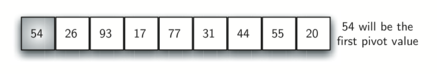
\includegraphics[width=0.8\columnwidth]{fig/firstsplit.png}
%     % \caption{Choose pivot}
%     \label{fig:choose_pivot}
%     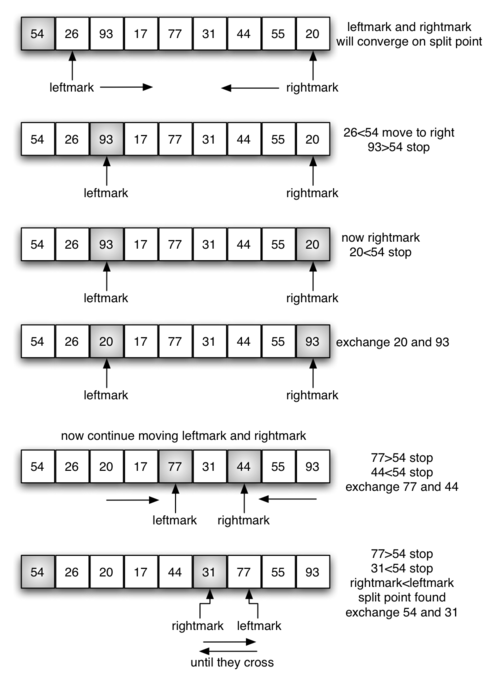
\includegraphics[width=0.8\columnwidth]{fig/partitionA.png}
%     \caption{Hoarse Partition}
% \end{figure}
% Python code:
% \begin{lstlisting}[language= Python]
% def quickSort(alist):
%   quickSortHelper(alist,0,len(alist)-1)

% def quickSortHelper(alist,first,last):
%   if first<last:

%       splitpoint = partition(alist,first,last)

%       quickSortHelper(alist,first,splitpoint-1)
%       quickSortHelper(alist,splitpoint+1,last)

% alist = [54,26,93,17,77,31,44,55,20,100]
% quickSort(alist)
% print(alist)
% \end{lstlisting}

\subsubsection{Lomuto's Partition}
\begin{figure}[!ht]
    \centering
    % 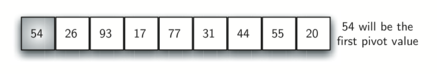
\includegraphics[width=0.8\columnwidth]{fig/firstsplit.png}
    % \caption{Choose pivot}

    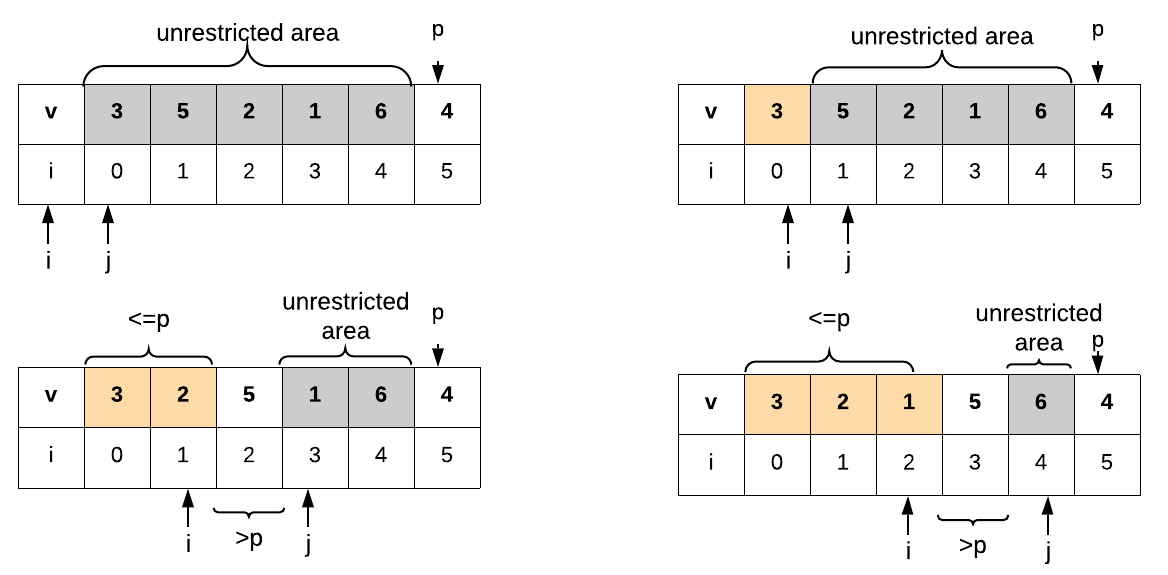
\includegraphics[width=0.98\columnwidth]{fig/quicksort.png}
    \caption{Lomuto's Partition. Yellow, while, and gray marks as region (1), (2) and (3), respectively.}
        \label{fig:lumo_partition}
\end{figure}
We use example $A=[3, 5, 2, 1, 6, 4]$ to demonstrate this partition method. Assume our given range for partition is $[s, e]$, and  $p = A[e]$ is chosen as pivot. We would use two pointer technique $i, j$ to maintain three regions in subarray $A[s, e]$: (1) region $[s, i]$ with items smaller than or equal to $p$;  (2) $[i+1, j-1]$ region with item larger than $p$; (3) unrestricted region $[j, e-1]$.  These three areas and the partition process on the example is shown in Fig.~\ref{fig:lumo_partition}. 

\begin{itemize}
    \item At first, $i=s-1, j = s$. Such initialization guarantees that region (1) and (2) are both empty, and region (3) is the full range other than the pivot. \item Then, scan scan items in the unrestricted area using pointer $j$:
    \begin{itemize}
        \item If the current item $A[j]$ belongs to region (2), that is to say $A[j] >  p$,  we just increment pointer $j$; 
        \item Otherwise when $A[j] <= p$, this item should goes to region (1). We accomplish this by swapping this item with the first item in region (2) at $i+1$. And now region (1) increments by one and region (2) shifts one position backward.  
    \end{itemize}
    \item After the for loop, we need to put our pivot at the first place of region (2) by swapping. And now, the whole subarray is successfully parititioned into three regions as we needed, and return where the index of where the pivot is at--$i+1$--as the partition index. 
\end{itemize}
We The implementation of as follows:
\begin{lstlisting}[language = Python]
def partition(a, s, e):
  p = a[e]
  i = s - 1
  # Scan unresticted area
  for j in range(s, e): 
    # Swap 
    if a[j] <= p:
      i += 1
      a[i], a[j] = a[j], a[i] 
  a[i+1], a[e] = a[e], a[i+1]
  return i+1
\end{lstlisting}

% \subsubsection{Hoare Partition}
% In hoare partition, $i$ is placed at the same place as in the Lumoto's partition, and j starts at $e$ and $i$ and $j$ move towards each other. The regions are: $A[p...i] \le x, A[i+1...j-1], A[j...e-1]>x$.  When we are at position $j-1$, we compare this item with pivot, if it is larger than x, we decrease $j$. For i, if it is smaller than or equal to x, we increase $i$. Until there are both violation at $i$ and $j$, we swap these two items.  Also, $j$ stops when $j=i$. 
% \begin{lstlisting}[language = Python]
% def HoarePartition(arr,low,high):
%     pivot=arr[high]
%     i=low
%     j=high-1
%     while True:
%         while arr[i] <= pivot and i < j:
%             i += 1
%         while arr[j] >= pivot and i < j:
%             j -= 1
%         if i == j:
%             if arr[i] <= pivot:
%                 i += 1
%             arr[i], arr[high] = arr[high], arr[i]
%             return i
%         else:
%             arr[i], arr[j] = arr[j], arr[i]
% \end{lstlisting}
\paragraph{Complexity Analysis} The worst case of the partition appears when the input array is already sorted or is reversed from the sorted array. In this case, it will partition a problem with size $n$ into one subproblem with size $n-1$ and the other subproblem is just empty. The recurrence function is $T(n) = T(n-1) + O(n)$, and it has a time complexity of $O(n^2)$. And the best case appears when a subprocess is divided into half and half as in the merge sort, where the time complexity is $O(n\log n)$. Randomly picking the pivot from $A[s, e]$ and swap it with $A[e]$ can help us achieve a stable performance with average $O(n\log n)$ time complexity.
\subsubsection{Stablity of Quick Sort} Quick sort is \textit{not stable}, because there are cases items can be swapped no matter what: (1) as the first item in the region (2), it can be swapped to the end of region (2). (2) as the pivot, it  is swapped with the first item in the region (2) too. Therefore, it is hard to guarantee the stability among equal keys. We can try experiment with $A = [(2, 1), (2, 2), (1, 1)]$, and use the first element in the tuple as key. This will sort it as $A=[(1, 1), (2, 2), (2, 1)]$.

However, we can still make quick sort stable if we get rid of the swaps by using two extra lists: one for saving the smaller and equivalent items and the other for the larger items. 
%%%%%%%%%%%%%%%%%%%%%%%%Quick Select$$$$$$$$$$$$$$$$$$
\subsubsection{Quick Select} 
Quick Select is a variant of quick sort, and it is used   to find the $k$-th smallest item in a list in linear time.  In quicksort,  it recurs  both sides of the partition index, while in quick select, only the side that contains the $k$-th smallest item will be recurred. This is similar to the binary search, the comparison of $k$ and partition index $p$ results three cases:
\begin{itemize}
    \item If $p=k$, we find the $k$-th smallest item, return. 
    \item If $p > k $, then we recur on the right side.
     \item If $p < k $, then we recur on the left side.
\end{itemize}
Based on the structure, quick select has the following recurrence time complexity function:
\begin{align}
T(n) &= T(n/2) + O(n)\\ 
T(n) &= O(n) \texttt{ (with master theorem)}
\end{align}
% This reduces the expected complexity from $O(n \log n)$ to $O(n)$, with a worst case of $O(n^2)$.
\paragraph{Implementation} We first set $k$ in range of $[s, e]$. When $s=e$, there is only one item in the list, which means we no longer can divide it. This is our end condition and is also the case when our original list has only one item, then we have to return this item as the 0-th smallest item. 
\begin{lstlisting}[language=Python]
def quickSelect(a, s, e, k, partition=partition):
  if s >= e:
    return a[s]

  p = partition(a, s, e) 
  if p == k:
    return a[p]
  if k > p:
    return quickSelect(a, p+1, e, k, partition)
  else:
    return quickSelect(a, s, p-1,  k, partition)
\end{lstlisting}




%%%%%%%%%%%%%%%%
% Section: Counting sort %
%%%%%%%%%%%%%%%%
\section{Linear Sorting}
\label{linear_sorting}
Sorting  without basing upon comparisons is possible, creative, and even faster, proved by the three non-comparative sorting algorithms we are about to introduce: Bucket Sort, Counting Sort, and Radix Sort. 
For these algorithms the theoretic lower bound $O(n\log n)$ of comparison-based sorting is not likewise a lower bound any more; they all work in linear time. However, there are limitations to the input data, as these sorting techniques  rely on certain assumptions concerning the data to be sorted to be able to work. 

Although the three algorithms we see in this section come in different forms and rely on different assumptions to the input data, we see one thing in common: They all use the divide and conquer algorithm design paradigm. Let's explore their unique tricks and the restrictive applications!

\subsection{Bucket Sort}
Bucket Sort assumes that the input data satisfying a uniform distribution. The uniform distribution  is usually assumed to be in interval $[0, 1)$. However, it can be extended to any uniform distribution with simple modification. Bucket sort applies a one time divide and conquer trick--it divides the input data into $n$ independent segments, $n$ the size of the input, just as what we have seen in merge sort, and then insertion sort is applied on each segment, and finally each sorted segmented is combined to get the result. 

Bucket sort manages the dividing process by assigning $n$ empty \textbf{buckets}, and then distribute the input data $a[i]$ to bucket index \texttt{int(a[i]*n)}. For example, if $n=10$, and $a[i]=0.15$, the bucket that the number goes to is the one with index $1$. We use example a = [0.42, 0.72, 0.  , 0.3 , 0.15, 0.09, 0.19, 0.35, 0.4 , 0.54], and visualize the process in Fig.~\ref{fig:bucket_sort}. 
\begin{figure}[!ht]
    \centering

    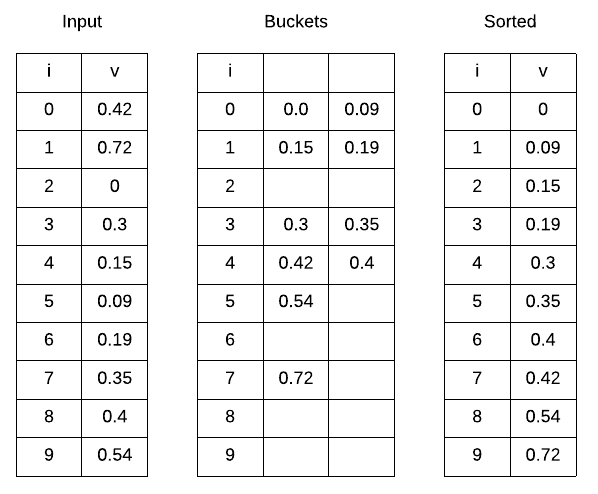
\includegraphics[width=0.8\columnwidth]{fig/bucket_sort.png}
    \caption{Bucket Sort}
        \label{fig:bucket_sort}
\end{figure}


\paragraph{Implementation} First, we prepare the input data with \texttt{random.uniform} from \texttt{numpy} library. For simplicity and the reconstruction of the same input, we used random seed and rounded the float number to only two decimals.
\begin{lstlisting}[language=Python]
import numpy as np
np.random.seed(1)
a = np.random.uniform(0,  1, 10)
a = np.round(a, decimals=2)
\end{lstlisting}
Now, the code for the bucket sort is straightforward as:
\begin{lstlisting}[language=Python]
from functools import reduce
def bucketSort(a):
  n = len(a)
  buckets = [[] for _ in range(n)]
  # Divide numbers into buckets
  for v in a:
    buckets[int(v*n)].append(v)
  # Apply insertion sort within each bucket
  for i in range(n):
    insertionSort(buckets[i])
  # Combine sorted buckets
  return reduce(lambda a, b: a + b, buckets)
\end{lstlisting}
\paragraph{Complexity Analysis} 
\paragraph{Extension} To extend to uniform distribution in any range, we first find the minimum and maximum value, $minV, maxV$, and  compute the bucket index $i$  for number $a[i]$ with formula:
\begin{align}
i= n\frac{a[i]-minV}{maxV-minV} 
\end{align}
\subsection{Counting Sort}
\label{O_n_k_sorting}
Counting sort is an algorithm that sorts items according to their corresponding keys that are small integers. It works by counting the occurrences of each distinct key value, and using arithmetic--prefix sum--on those counts to determine the position of each key value in the sorted sequence.  Counting sort no longer fits into the comparison-based sorting paradigm because it uses the keys as indexing to assist the sorting instead of comparing them directly to decide  relative positions. For input that comes with size $n$ and the difference between the maximum and minimum integer keys $k$, counting sort has a time complexity $O(n+k)$.






% The counting sort is a sorting technique based on keys between a specific range. It works by counting the occurrence number of each distinct key and saves it into a count array. Then a prefix sum computation is applied on count array. Eventually, a loop over the given array and put the key to location pointed out by the count array. 
\subsubsection{Premise: Prefix Sum} Before we introduce counting sort, first let us see what is prefix sum. Prefix sum, a.k.a cumulative sum, inclusive scan, or simply scan of a sequence of numbers $x_i, i \in [0, n-1]$ is  second sequence of numbers $y_i, i \in [0, n-1]$, and $y_i$ is the sums of prefixes of the input sequence, with equation:
\begin{align}
 y_i = \sum_{j=0}^ix_j   
\end{align}
For instance, the prefix sums of on the following array is: 
\begin{lstlisting}[numbers=none]
Index: 0  1  2  3  4  5
x:     1  2  3  4  5  6
y:     1  3  6  10 15 21
\end{lstlisting}

Prefix sums are trivial to compute with the following simple recurrence relation  in $O(n)$ complexity. 
\begin{align}
    y_i = y_{i-1} + x_i, i \geq 1
\end{align}

Despite the ease of computation, prefix sum is a useful primitive in certain algorithms such as counting sort and Kadane's Algorithm as you shall see through this book. 

\subsubsection{Counting Sort}
Given an input array $[1, 4, 1, 2, 7, 5, 2]$, let's see how exactly counting sort works by explaining it in three steps. Because our input array comes with duplicates, we distinguish the duplicates by their relative order shown in the parenthesises. Ideally, for this input, we want it to be sorted as:
\begin{lstlisting}[numbers=none]
Index: 0     1    2     3    4  5  6
Key:   1(1)  4   1(2)  2(1)  7  5  2(2)
Sorted:1(1) 1(2) 2(1)  2(2)  4  5  7
\end{lstlisting}
\begin{figure}[!ht]
    \centering

    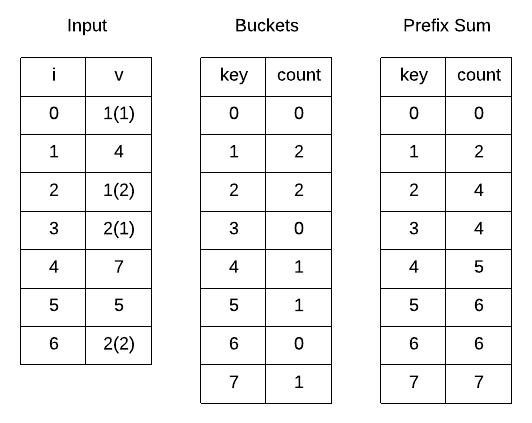
\includegraphics[width=0.8\columnwidth]{fig/counting_sort_1.png}
    \caption{Counting Sort: The process of counting occurrence and compute the prefix sum.}
        \label{fig:counting_sort_1}
\end{figure}
\begin{enumerate}
    \item \textbf{Count Occurrences:} We assign a \texttt{count} array $C_i$, and assign a size 8, which has index in range $[0, 7]$ and will be able to contain our keys whose range is $[1, 7]$.  which has the same size of the key range $k$. We loop over each key in the input array, and use key as index to  count each key's occurrence. Doing so will get the following result. And it means in the input array, we have two 1's, two 2's, one 4, one 5, and one 7. The process is shown in Fig.~\ref{fig:counting_sort_1}.
    
    Counting sort is indeed a subtype of bucket sort, where the number of buckets is $k$, and each bucket stores keys implicitly by using keys as indexes and the occurrence to track the total number of the same keys. 
% \begin{lstlisting}[numbers=none]
% Index:     0  1  2  3  4  5  6  7
% Count:     0  2  2  0  1  1  0  1
% \end{lstlisting}

\item \textbf{Prefix Sum on Count Array:} We compute the prefix sum for \texttt{count} array, which is shown as:
\begin{lstlisting}[numbers=none]
Index:          0  1  2  3  4  5  6  7
Count:          0  2  2  0  1  1  0  1
Prefix Sum:     0  2  4  4  5  6  6  7
\end{lstlisting}
Denote the prefix sum array as $ps$. For key $i$, $ps_{i-1}$ tells us the number of items that is less or equals to ($\leq$) key $i$. This information can be used to place key $i$ directly into its correct position. For example, for key 2, summing over its previous keys' occurrences ($ps_{1})$ gives us 2, indicating that we can put key 2 to position $2$. However, key 2 appears two times, and the last position of key 2 is indicated by $ps_2 - 1$, which is 3.  Therefore, for any key $i$, its locations in the sorted array is in range $[ps_{i-1}, ps_i)$. 
%Observing the count array after this step showing in the below table, key 7 will be the order $(C_6, C_7]$, which is $(6, 7]$, that is only the 7-th position at index 6. For key 2, it is in the range of $(2, 4]$, that is 3-th and 4-th position. 
% \begin{lstlisting}[numbers=none]
% Index:          0  1  2  3  4  5  6  7
% Prefix Sum:     0  2  4  4  5  6  6  7
% \end{lstlisting}
We could have just scan the prefix sum array, and use the prefix sum as locations for key indicated by index of prefix sum array. However, this method is only limited to  situations where the input array is integers. Moreover, it is unable to keep the relative ordering of the items of the same key. 

\item \textbf{Sort Keys with Prefix Sum Array: }  First, let us loop over the input keys from position $0$ to $n-1$. For $key_i$, we decrease the prefix sum by one, $ps_{key_i} = ps_{key_i}-1$ to get the last position that we can assign this key in the sorted array. The whole process is shown in Fig.~\ref{fig:counting_sort}. We saw that items of same keys are sorted in reverse order. Looping over keys in the input in reverse order is able to  correct this and thus making the counting sort a stable sorting algorithm. 
\begin{figure}[!ht]
    \centering
    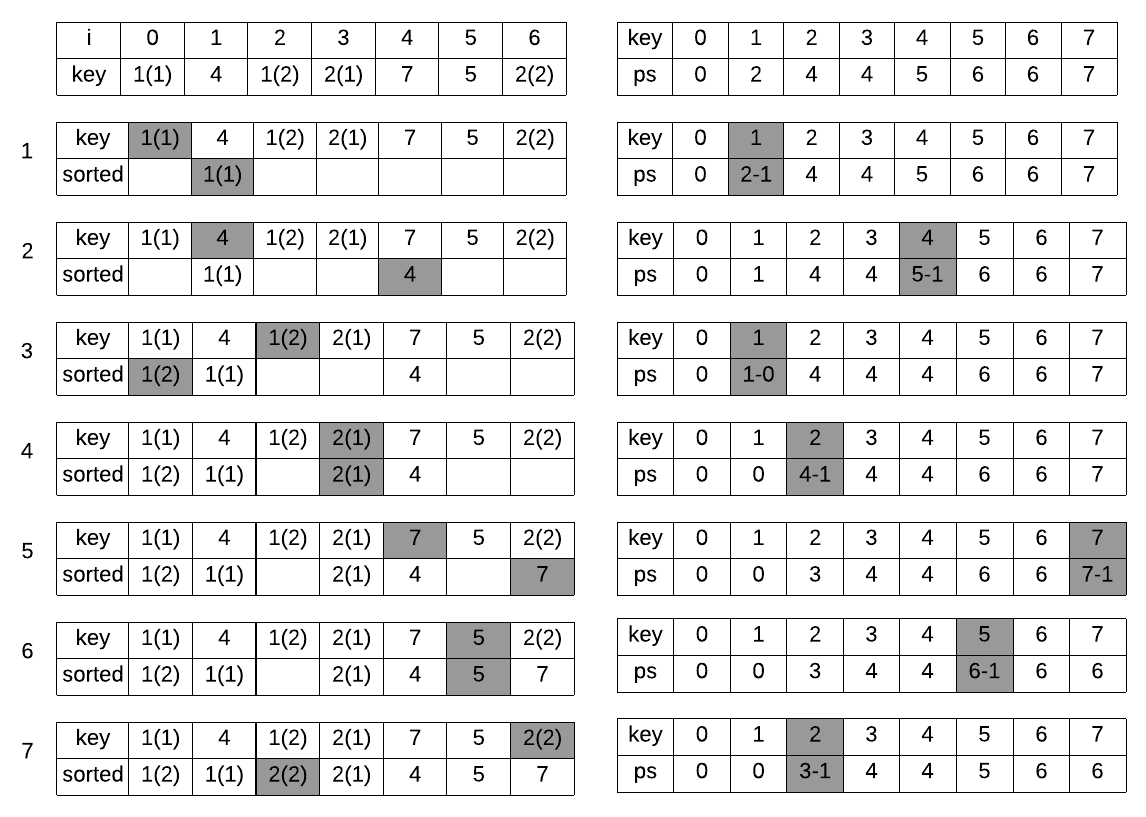
\includegraphics[width=1.1\columnwidth]{fig/counting_sort.png}
    \caption{Counting sort: Sort keys according to prefix sum.}
        \label{fig:counting_sort}
\end{figure}

\end{enumerate}
 
 
\paragraph{Implementation} In our implementation, we first find the range of the input data, say it is $[minK, maxK]$, making our range $k = maxK-minK$. And we recast the key as $key - minK$ for two purposes:
\begin{itemize}
    \item To save space for \texttt{count} array.
    \item To be able to handle negative keys.
\end{itemize}The implementation of the main three steps are  nearly the same as what we have discussed other than the recast of the key. In the process, we used two auxiliary arrays:  \texttt{count} array for counting and accumulating the occurrence of keys with $O(k)$ space and \texttt{order} array for storing the sorted array with $O(n)$ space, giving us the space complexity $O(n+k)$ in our implementation. The Python code is shown as:
\begin{lstlisting}[language=Python]
def countSort(a):
  minK, maxK = min(a), max(a)
  k = maxK - minK + 1
  count = [0] * (maxK - minK + 1)
  n = len(a)
  order = [0] * n
  # Get occurrence
  for key in a:
    count[key - minK] += 1
  
  # Get prefix sum
  for i in range(1, k):
    count[i] += count[i-1]
    
  # Put key in position
  for i in range(n-1, -1, -1):
    key = a[i] - minK
    count[key] -= 1 # to get the index as position
    order[count[key]] = a[i] 
  return order
\end{lstlisting}

\paragraph{Properties} Counting sort is \textbf{out-of-place} for the auxiliary \texttt{count} and \texttt{order} array.  Counting sort is \textbf{stable} given that we iterate keys in  the input array in reversed order.  Counting sort is likely to have $O(n+k)$  for both the space and time complexity. 

\paragraph{Applications} Due to the special character that counting sort sorts by using key as index, and the range of keys decides the time and space complexity, counting sort's applications are limited. We list the most common applications:
\begin{itemize}
    \item Because the time complexity depends on the size  of $k$, in practice counting sort is usually used when $k=O(n)$, in which case it makes the time complexity $O(n)$. 
    \item Counting sort is often used  as a sub-routine. For example, it is a part of other sorting algorithms such as radix sort, which is a linear sorting algorithm. We will also see some examples in string matching chapter.  
\end{itemize}

\subsection{Radix Sort}
The word ``Radix'' is a mathematical term for the \textit{base} of a number. For example, decimal and hexadecimal number has a radix of 10 and 16, respectively. For strings of alphabets has a radix of 26 given there are 26 letters of alphabet. Radix sort is a non-comparative sorting methods that utilize the concept of radix or base to  order a list of integers digit by digit or a list of strings letter by letter.  The sorting of integers or strings of alphabets is different based on the different concepts of ordering--number ordering and the lexicographical order as we have introduced. We show one example for list of integers and strings and their sorted order or lexicographical order: 
%the sorted order for [170, 45, 75, 90, 802, 24] is [24, 45, 75, 90, 170, 802]. For a list of fruits [apple, pear, berry, peach, apricot], its lexicographical order is [apple, apricot, berry, peach, pear]. 
\begin{lstlisting}[numbers=none]
Integers: 170, 45, 75, 90, 802, 24
Sorted:   24, 45, 75, 90, 170, 802
\end{lstlisting}

\begin{lstlisting}[numbers=none]
Strings: apple, pear, berry, peach, apricot
Sorted:  apple, apricot, berry, peach, pear
\end{lstlisting}
And we see how that the integers are ordered by the length of digits, whereas in the sorted strings, the length of strings does not usually decide the ordering. 

Within Radix sorting, it is  usually either the bucket sort or counting sort that is doing the sorting using one radix as key at a time. Based upon the sorting order of the digit, we have two types of radix sorting: \textit{Most Significant Digit (MSD) radix sort} which starts from the left-most radix first and goes all the way the right-most radix, and \textit{Least Significant Digit (LSD) radix sort} vice versa.  
% \begin{itemize}
%     \item In our fruit alphabetization example,  it groups the strings by a single letter with either bucket sort or counting sort under the hood,  starting from the very first letter on the left side all the way to the very last on the right if necessary. This form of radix sort is also know as Most Significant Digit (MSD) radix sort, and is usually solved by recursion. 
%     \item 
% \end{itemize}
We should address the details of the two forms of radix sort -- MSD and LSD using our two examples. 

\subsubsection{LSD Radix Sorting Integers} 
LSD radix sort is often used to sort list of integers.  It  sorts the entire numbers one digit/radix at a time from the least-significant to the most-significant digit. For a list of positive integers where the maximum of them has $m$ digits, LSD radix sort takes a total of $m$ passes to finish sorting. 

\begin{figure}[!ht]
    \centering
    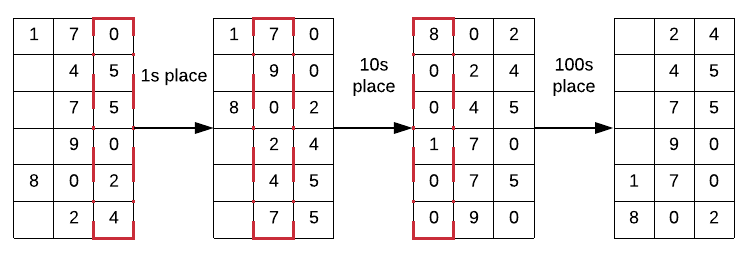
\includegraphics[width=0.98\columnwidth]{fig/lsd_radix_integer_sort.png}
    \caption{Radix Sort: LSD sorting integers in iteration}
        \label{fig:lsd_radix_integer_sort}
\end{figure}

Here, we demonstrate the process of LSD radix sorting on our exemplary list of integers with counting sort as a subroutine to sort items by using each radix as key. $m=3$ in our example:
\begin{itemize}
    \item As shown in Fig.~\ref{fig:lsd_radix_integer_sort}, in the first pass, the least significant digit (1st place) is used as key to sort.  After this pass, the ordering of numbers of unit digits is in-place. 
    \item In the second pass, the 10s place digit is used. After this pass, we see that numbers that has less than or equals to two digits comprising $24, 45, 75, 90$ in our example is in ordering. 
    \item At the last and third pass, the 100s place digit is used. For numbers that are short of 100s place digit, 0 is placed. Afterwards, the entire numbers are in ordering. 
\end{itemize}
We have to notice that the sorting will not work unless the sorting subroutine we apply is stable. For example, in our last pass, there exists four zeros, indicating that they share the same key value. If the relative ordering of them is not kept, the previously sorting effort will be wasted. 
\paragraph{Implementation}
To implement the code with Python, we first need to know how to get each digit out of an integer. With number 178 as an example:
\begin{itemize}
    \item The  least significant digit 8 is the reminder of $178\%10$. 
    \item The second least-significant digit 7 is the reminder of $17\%10$.
    \item And the most-significant digit 1 is the reminder of $1\%10$.
\end{itemize}
As we see for digit 8, we need to have 178, for digit 7, we need to have 17, and for digit 1, we only need 1. $178, 17, 1$ are the prefix till the digit we need. We can obtain these prefixes via a base $exp$.
\begin{lstlisting}[numbers=none]
exp = 1, (178 // exp ) = 178, 178 % 10 = 8
exp = 10, (178 // exp ) = 17, 17 % 10 = 7
exp = 100, (178 // exp ) = 1, 1 % 10 = 1
\end{lstlisting}
We can also get the prefix by looping and each time we divide our number by 10. For example, the following code will output [8, 7, 1]. 
\begin{lstlisting}[language = Python]
a = 178
digits = []
while a > 0:
    digits.append(a%10)
    a = a // 10
\end{lstlisting}
Now, we know the number of loops we need is decided by the maximum positive integer in our input array. On the code basis, we use a \texttt{while} loop to obtain the prefix and making sure that it is larger than 0. At each pass, we call \texttt{count\_sort} subroutine to sort the input list. The code is shown as:
\begin{lstlisting}[language=Python]
def radixSort(a):
  maxInt = max(a)
  exp = 1
  while maxInt // exp > 0:
    a = count_sort(a, exp)
    exp *= 10
  return a
\end{lstlisting}
For subroutine \texttt{count\_sort} subroutine, it is highly similar to our previously implemented counting sort but two minor differences:
\begin{itemize}
    \item Because  we sort by digits, therefore, we have to use a formula: $key = (key // exp) \% 10$ to covert the key to digit. 
    \item Because for decimal there are in total only 10 digits, we only arrange 10 total space for the \texttt{count} array. 
\end{itemize}
The code is as:
\begin{lstlisting}[language=Python]
def count_sort(a, exp):
  count = [0] * 10 # [0, 9]
  n = len(a)
  order = [0] * n
  # Get occurrence
  for key in a:
    key = (key // exp) % 10
    count[key] += 1
  
  # Get prefix sum
  for i in range(1, 10):
    count[i] += count[i-1]
    
  # Put key in position
  for i in range(n-1, -1, -1):
    key = (a[i] // exp) % 10
    count[key] -= 1 # to get the index as position
    order[count[key]] = a[i] 
  return order
\end{lstlisting}
\paragraph{Properties and Complexity Analysis} 
Radix sorting for integers takes $m$ passes with $m$ as the total digits, and each pass takes $O(n+k)$, where $k=10$ since there is only 10 digits for decimals. This gives out a total of $O(mn)$ time complexity, and $m$ is rather of a constant compared with variable $n$, thus radix sorting for integers with counting sort as subroutine has a linear time complexity. Due to the usage of counting sort, which is stable, making the radix sorting a stable sorting algorithm too.

With  the usage of auxiliary \texttt{count} and \texttt{order}, it gives a $O(n)$ space complexity, and makes the LSD integer sorting an out-of- place sorting algorithm. 
\subsubsection{MSD Radix Sorting Strings}
In our fruit alphabetization example,  it uses MSD radix sorting and groups the strings by a single letter with either bucket sort or counting sort under the hood,  starting from the very first letter on the left side all the way to the very last on the right if necessary. MSD radix sorting is usually implemented with recursion. 

\begin{figure}[!ht]
    \centering
    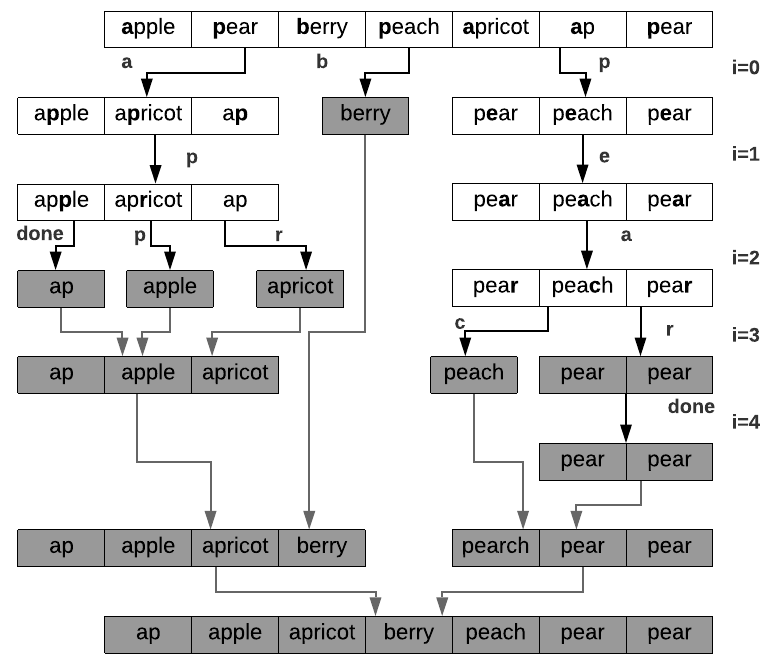
\includegraphics[width=0.9\columnwidth]{fig/msd_radix_string_sort.png}
    \caption{Radix Sort: MSD sorting strings in recursion. The black and grey arrows indicate the forward and backward pass in recursion, respectively. }
        \label{fig:msd_radix_string_sort}
\end{figure}

For better demonstration, we add two more strings: ``ap'' and ``pear''. String ``ap'' is for showing what happens when the strings in the same bucket but one is shorter and has no valid letter to compare with. And string ``pear'' is to showcase how the algorithm handles duplicates. 
The algorithm  indeed applies the recursive divide and conquer design methodology. 

\paragraph{Implementation} We show bucket sort here, as in lexicographical ordering, the first letter of the strings already decide the ordering of groups of strings bucketed by this letter. This LSD sorting method divide the strings into different buckets indexed by letter, and it then combines the returned results together to get the final sorted strings, which is highly similar to merge sort.  %the groups of strings by the first letter but in our code source, the one with counting sort is provided too. 
\begin{itemize}
    \item At first, the recursion handles the first keys of the first letter in the string, as the process where $i=0$ shown in Fig.~\ref{fig:msd_radix_string_sort}. There are three buckets with letter `a', `b', and `p'. 
    \item At depth 2 when $i=1$, the resulting buckets from depth 1 is further bucketed by the second letter. Bucket `b' contains only one item, which itself is sorted, thus, the recursion end for this bucket. For the last bucket `a' and `p', they are further bucketed by letter `p' and `e'. 
    \item At depth 3 when $i=2$, for the last bucket `p', it further results two more buckets `p' and `r'. However, for string `ap' in the bucket, there is no valid third letter to use as index. And according to the lexicographical order, it puts `ap' in earlier ordering of the resulted buckets. \item In our example, the forward process in the recursion is totally done when $i=4$. It then enters into the backward phase, which merges buckets that are either composed of a single item or the \texttt{done\_bucket}. 
\end{itemize}

The code is offered as:
\begin{lstlisting}[language=Python]
def MSD_radix_string_sort(a, i):
  # End condition: bucket has only one item
  if len(a) <= 1:
    return a

  # Divide
  buckets = [[] for _ in range(26)]
  done_bucket = []
  for s in a:
    if i >= len(s):
      done_bucket.append(s)
    else:
      buckets[ord(s[i]) - ord('a')].append(s)
  # Conquer and chain all buckets
  ans = []
  for b in buckets:
    ans += MSD_radix_string_sort(b, i + 1)
  return done_bucket + ans
\end{lstlisting}

\paragraph{Properties and Complexity Analysis} 
Because the bucket sort itself is a stable sorting algorithm, making the radix sort for string stable too.

The complexity analysis for the recursive Radix sorting can be accomplished with recursion tree. The tree has nearly $n$ leaves. The worst case occurs when all strings within the input array are the same, thus the recursion tree degrades to linear structure with length $n$ and within each node $O(n)$ is spent to scan items of corresponding letter, making the worst time complexity $O(n^2)$.  

For the existence of auxiliary \texttt{buckets}, \texttt{done\_bucket}, and \texttt{ans} arrays in sorting of strings, it is an out-of-place sorting. With the same recursion tree analysis for space, we have linear space complexity too. 

% The connection of BST/Trie to Quciksort/Radix Sort. 

% \textcolor{red}{Need further understanding}. A binary search tree is a dynamic version of what happens during quicksort. The root represents an arbitrary (but hopefully not too far off from the median) pivot element from the collection. The left subtree is then everything less than the root, and the right subtree is everything greater than the root. The left and right collections are then again ordered in the same manner, i.e. the data structure is defined recursively.

% A trie is a dynamic version of what happens during radix sort. You look at the first bit or digit of a number (or first letter of a string) to determine which subtree the value belongs in. You then repeat the procedure recursively using the next character or digit to determine which of the subtree's children it belongs in, and so on.


% %%%%%%%%%%%%%%%%
% % Section: bucket sort %
% %%%%%%%%%%%%%%%%
% \section{$O(n)$ Sorting}
% \label{o_n_sorting}


% \paragraph{Use Counting Sort} Counting sort is one of the most efficient sorting algorithm for lexicographical ordered sorting. 
% \begin{lstlisting}[language = Python]
% def countSort(arr):
 
%     # The output character array that will have sorted arr
%     output = [0 for i in range(256)]
 
%     # Create a count array to store count of inidividul
%     # characters and initialize count array as 0
%     count = [0 for i in range(256)]
 
%     # For storing the resulting answer since the 
%     # string is immutable
%     ans = ["" for _ in arr]
 
%     # Store count of each character
%     for i in arr:
%         count[ord(i)] += 1
 
%     # Change count[i] so that count[i] now contains actual
%     # position of this character in output array
%     for i in range(256):
%         count[i] += count[i-1]
 
%     # Build the output character array
%     for i in range(len(arr)):
%         output[count[ord(arr[i])]-1] = arr[i]
%         count[ord(arr[i])] -= 1
 
%     # Copy the output array to arr, so that arr now
%     # contains sorted characters
%     for i in range(len(arr)):
%         ans[i] = output[i]
%     return ans 
 
% # Driver program to test above function
% arr = "geeksforgeeks"
% ans = countSort(arr)
% print "Sorted character array is %s"  %("".join(ans))
% \end{lstlisting}


%%%%%%%%%%%%%%%%
% Section: Python sort %
%%%%%%%%%%%%%%%%
\section{Python Built-in Sort}
\label{python_built_in_sort}
There are two built-in functions to sort \texttt{list} and other iterable objects in Python 3, and both of them are stable. In default, they use \texttt{<} comparisons between items and sort items in increasing order. 
\begin{itemize}
    \item Built-in method \texttt{list.sort(key=None, reverse=False)} of \texttt{list} which sorts the items in the list in-place, and returns \texttt{None}.
    \item Built-in function \texttt{sorted(iterable, key=None, reverse=False)} works on \textit{any iterable object}, including \texttt{list}, \texttt{string}, \texttt{tuple}, \texttt{dict}, and so on. It sorts the items out-of-place; returning another \texttt{list} and keeps the original input unmodified. 
\end{itemize}
\subsubsection{Basics}
To use the above two built-in methods to sort a list of integers is just as simple as:
\begin{lstlisting}[language=Python]
lst = [4, 5, 8, 1, 2, 7]
lst.sort()
\end{lstlisting}
Printing out \texttt{lst} shows that the sorting happens in-place within \texttt{lst}. 
\begin{lstlisting}[language=Python]
[1, 2, 4, 5, 7, 8]
\end{lstlisting}
Now, use \texttt{sorted()} for the same list:
\begin{lstlisting}[language=Python]
lst = [4, 5, 8, 1, 2, 7]
new_lst = sorted(lst)
\end{lstlisting}
We print out:
\begin{lstlisting}[language=Python]
new_lst, lst
([1, 2, 4, 5, 7, 8], [4, 5, 8, 1, 2, 7])
\end{lstlisting}
Let's try to sort other iterable object, and try sort a tuple of strings:
\begin{lstlisting}[language=Python]
fruit = ('apple', 'pear', 'berry', 'peach', 'apricot')
new_fruit = sorted(fruit)
\end{lstlisting}
Print out \texttt{new\_fruit}, and we also see that it returned a \texttt{list} instead of \texttt{tuple}.
\begin{lstlisting}[language=Python]
['apple', 'apricot', 'berry', 'peach', 'pear']
\end{lstlisting}
Note: For \texttt{list}, \texttt{list.sort()} is faster than \texttt{sorted()} because it doesn't have to create a copy. For any other iterable, we have no choice but to apply \texttt{sorted()} instead.

\paragraph{Change Comparison Operator} What if we want to redefine the behavior of comparison operator \texttt{<}? Other than writing a class and defining \texttt{\_\_lt\_\_()}, in Python 2, these two built-in functions has another argument, \texttt{cmp}, but it is totally dropped in Python 3. We can use \texttt{functools}'s \texttt{cmp\_to\_key} method to convert to key in Python 3. For example, we want to sort [4, 5, 8, 1, 2, 7] in reverse order, we can define a \texttt{cmp} function that reverse the order of items to be compared:
\begin{lstlisting}[language=Python]
def cmp(x, y):
  return y - x
\end{lstlisting}
And then we call this function as:
\begin{lstlisting}[language=Python]
from functools import cmp_to_key
lst.sort(key=cmp_to_key(cmp))
\end{lstlisting}
The printout of \texttt{lst} is:
\begin{lstlisting}[language=Python]
[8, 7, 5, 4, 2, 1]
\end{lstlisting}

\paragraph{Timsort}
These two methods both using the same sorting method -- \textit{Timsort} and has the same parameters. Timesort is a hybrid stable and in-place sorting algorithm, derived from merge sort and insertion sort, designed to perform well on many kinds of real-world data. It uses techniques from Peter McIlroy's ``Optimistic Sorting and Information Theoretic Complexity'', January 1993. It was implemented by Tim Peters in 2002 for use in the Python programming language. The algorithm finds subsequences of the data that are already ordered, and uses that knowledge to sort the remainder more efficiently.

\subsubsection{Arguments}
They both  takes two keyword-only arguments: \texttt{key} and \texttt{reverse}:, and each has \texttt{None} and \texttt{False} as default value, respectively. 
\begin{itemize}
    \item Argument \texttt{key}: ot specifies a function of one argument that is used to extract a comparison key from each list item (for example, \texttt{key=str.lower}). If not set, the default value \texttt{None} means that the list items are sorted directly. 
    \item Argument \texttt{reverse}: a boolean value.  If  set to \texttt{True}, then the list or iterable is sorted as if each comparison were reversed(use \texttt{>=} sorted list is in Descending order. The dafault value is False. 
\end{itemize}
\paragraph{Sort in Reverse Order} Set \texttt{reverse=True} will sort a list of integers in decreasing order:
\begin{lstlisting}[language=Python]
lst = [4, 5, 8, 1, 2, 7]
lst.sort(reverse=True)
\end{lstlisting}
Print out \texttt{lst}, we see:
\begin{lstlisting}[language=Python]
[8, 7, 5, 4, 2, 1]
\end{lstlisting}
This is equivalent to customize a class \texttt{Int} and rewrite its \texttt{\_\_lt\_\_()} special method as:
\begin{lstlisting}[language=Python]
class Int(int):
  def __init__(self, val):
    self.val = val
  def __lt__(self, other):
    return other.val < self.val
\end{lstlisting}
Now, sort the same list but without setting \texttt{reverse} will get us exactly the same result:
\begin{lstlisting}[language=Python]
lst = [Int(4), Int(5), Int(8), Int(1), Int(2), Int(7)]
lst.sort()
\end{lstlisting}

\paragraph{Customize \texttt{key}}
We have mainly two options to customize the \texttt{key} argument: (1) through \texttt{lambda} function, (2) through a pre-defined function. And in either way, the function only takes one argument. For example, to sort the following list of tuples by using the second item in the tuple as key:
\begin{lstlisting}[language=Python]
lst = [(8, 1), (5, 7), (4, 1), (1, 3), (2, 4)]
\end{lstlisting}
We can write a function, and set \texttt{key} argument to this function
\begin{lstlisting}[language=Python]
def get_key(x):
  return x[1]
new_lst = sorted(lst, key = get_key)
\end{lstlisting}
The sorted result is:
\begin{lstlisting}[language=Python]
[(8, 1), (4, 1), (1, 3), (2, 4), (5, 7)]
\end{lstlisting}
The same result can be achieved via lambda function which is more convenient:
\begin{lstlisting}[language=Python]
new_lst = sorted(lst, key = lambda x: x[1])
\end{lstlisting}


Same rule applies to objects with named attributes. For example, we have the following class named \texttt{Student} that comes with three attributes: \texttt{name}, \texttt{grade}, and \texttt{age}, and we want to sort a list of \texttt{Student} class only through the age.
\begin{lstlisting}[language = Python]
class Student(object):
    def __init__(self, name, grade, age):
        self.name = name
        self.grade = grade
        self.age = age
    
    # To support indexing
    def __getitem__(self, key):
        return (self.name, self.grade, self.age)[key]

    def __repr__(self):
        return repr((self.name, self.grade, self.age))
\end{lstlisting}
We can do it through setting \texttt{key} argument still:
\begin{lstlisting}[language = Python]
students = [Student('john', 'A', 15), Student('jane', 'B', 12), Student('dave', 'B', 10)]
sorted(students, key=lambda x: x.age)
\end{lstlisting}
which outputs the following result:
\begin{lstlisting}[language=Python]
[('dave', 'B', 10), ('jane', 'B', 12), ('john', 'A', 15)]
\end{lstlisting}

The key-function patterns shown above are very common, so Python provides convenience functions to make accessor functions easier and faster. The \texttt{operator} module has \texttt{itemgetter()} and \texttt{attrgetter()} to get the attributes by index and name, respectively. For the sorting above, we can do it like this:
\begin{lstlisting}[language = Python]
from operator import attrgetter
sorted(students, key=attrgetter('age'))
\end{lstlisting}
\texttt{attrgetter} can take multiple arguments, for example, we can sort the list first by `grade' and then by `age', we can do it as:
\begin{lstlisting}[language = Python]
sorted(students, key=attrgetter('grade', 'age'))
\end{lstlisting}
which outputs the following result:
\begin{lstlisting}[language=Python]
[('john', 'A', 15), ('dave', 'B', 10), ('jane', 'B', 12)]
\end{lstlisting}
If our object supports indexing, which is why we defined \texttt{\_\_getitem\_\_()} in the class, we can use \texttt{itemgetter()} to do the same thing:
\begin{lstlisting}[language=Python]
from operator import itemgetter
sorted(students, key=itemgetter(2))
\end{lstlisting}


%%%%%%%%%%Summary and Bonus%%%%%%%%%%%%%%%%%%%%%
\section{Summary and Bonus}
Here, we give a comprehensive summary of the time complexity for different sorting algorithms.
\begin{figure}[h]
    \centering
    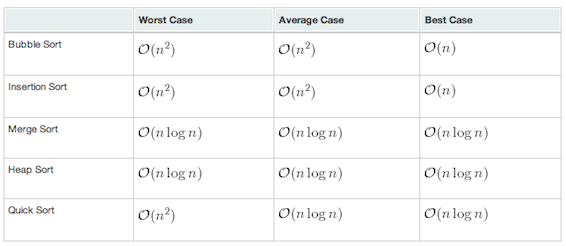
\includegraphics[width=1\columnwidth]{fig/time_complexity_sorting.png}
    \caption{The time complexity for common sorting algorithms}
    \label{fig:sort_complexity}
\end{figure}
%%%%%%%%%%exercise
\section{LeetCode Problems}

\paragraph{Problems}

\begin{examples}
    \item \textbf{Insertion Sort List (147).} Sort a linked list using insertion sort. A graphical example of insertion sort. The partial sorted list (black) initially contains only the first element in the list. With each iteration one element (red) is removed from the input data and inserted in-place into the sorted list
    
    Algorithm of Insertion Sort: Insertion sort iterates, consuming one input element each repetition, and growing a sorted output list.
    At each iteration, insertion sort removes one element from the input data, finds the location it belongs within the sorted list, and inserts it there. It repeats until no input elements remain. 
    \begin{lstlisting}[numbers=none]
Example 1:
Input: 4->2->1->3
Output: 1->2->3->4

Example 2:
Input: -1->5->3->4->0
Output: -1->0->3->4->5
    \end{lstlisting}
    
    \item \textbf{Merge Intervals (56, medium).} Given a collection of intervals, merge all overlapping intervals.
\begin{lstlisting}[numbers=none]
Example 1:
Input: [[1,3],[2,6],[8,10],[15,18]]
Output: [[1,6],[8,10],[15,18]]
Explanation: Since intervals [1,3] and [2,6] overlaps, merge them into [1,6].

Example 2:
Input: [[1,4],[4,5]]
Output: [[1,5]]
Explanation: Intervals [1,4] and [4,5] are considered overlapping.
\end{lstlisting}

\item \textbf{Valid Anagram (242, easy).} Given two strings s and t , write a function to determine if t is an anagram of s.
\begin{lstlisting}[numbers=none]
Example 1:
Input: s = "anagram", t = "nagaram"
Output: true

Example 2:
Input: s = "rat", t = "car"
Output: false
\end{lstlisting}
\textit{Note: You may assume the string contains only lowercase alphabets.}

Follow up: \textit{What if the inputs contain unicode characters? How would you adapt your solution to such case?}

\item \textbf{Largest Number (179, medium).}

\item \textbf{Sort Colors (leetcode: 75).} Given an array with n objects colored red, white or blue, sort them so that objects of the same color are adjacent, with the colors in the order red, white and blue. Here, we will use the integers 0, 1, and 2 to represent the color red, white, and blue respectively.
\textit{Note: You are not suppose to use the library's sort function for this problem.}

\item \textbf{ 
148. Sort List (sort linked list using merge sort or quick sort).}
\end{examples}

\paragraph{Solutions}
\begin{enumerate}
    \item Solution: the insertion sort is easy, we need to compare current node with all previous sorted elements. However, to do it in the linked list, we need to know how to iterate elements, how to build a new list. In this algorithm, we need two while loops to iterate: the first loop go through from the second node to the last node, the second loop go through the whole sorted list to compare the value of the current node to the sorted element, which starts from having one element. There are three cases for the comparison: if the comp\_node does not move, which means we need to put the current node in front the previous head, and the cur\_node become the new head; if the comp\_node stops at the back of it, so current node is the end, we set its value to 0, and we save the pre\_node in case; if it stops in the middle, we need to put cur\_node in between pre\_node and cur\_node. 
\begin{lstlisting}[language = Python]
def insertionSortList(self, head):
    """
    :type head: ListNode
    :rtype: ListNode
    """
    if head is None:
        return head
    sorted_head = head
    cur_node = head.next
    head.next = None #sorted list only has one node, a new list
    while cur_node:
        next_node = cur_node.next #save the next node
        cmp_node = head
        #compare node with previous all
        pre_node = None
        while cmp_node and cmp_node.val <= cur_node.val:
            pre_node = cmp_node
            cmp_node = cmp_node.next

        if cmp_node == head: #put in the front
            cur_node.next = head
            head = cur_node
        elif cmp_node == None: #put at the back
            cur_node.next = None #current node is the end, so set it to None
            pre_node.next = cur_node
            #head is not changed
        else: #in the middle, insert
            pre_node.next = cur_node
            cur_node.next = cmp_node
        cur_node = next_node
    return head
\end{lstlisting}

\item  Solution: Merging intervals is a classical case that use sorting. If we do the sorting at first, and keep track our merged intervals in a heap (which itself its sorted too), we just iterate into the sorted intervals, to see if it should be merged in the previous interval or just be added into the heap. Here the code is tested into Python on the Leetcode, however for the python3 it needs to resolve the problem of the heappush with customized class as iterable item.
\begin{lstlisting}[language = Python]
# Definition for an interval.
# class Interval(object):
#     def __init__(self, s=0, e=0):
#         self.start = s
#         self.end = e
from heapq import heappush, heappop

class Solution(object):
    def merge(self, intervals):
        """
        :type intervals: List[Interval]
        :rtype: List[Interval]
        """
        if not intervals:
            return []
        #sorting the intervals nlogn
        intervals.sort(key=lambda x:(x.start, x.end))
        h = [intervals[0]]
        # iterate the intervals to add
        for i in intervals[1:]:
            s, e = i.start, i.end
            bAdd = False
            for idx, pre_interal in enumerate(h):
                s_before, e_before = pre_interal.start, pre_interal.end
                if s <= e_before: #overlap, merge to the same interval
                    h[idx].end = max(e, e_before)
                    bAdd = True
                    break
            if not bAdd:
                #no overlap, push to the heap
                heappush(h, i)        
        return h
\end{lstlisting}

\item Solution: there could have so many ways to do it, the most easy one is to sort the letters in each string and see if it is the same. Or we can have an array of 26, and save the count of each letter, and check each letter in the other one string. 
\begin{lstlisting}[language = Python]
def isAnagram(self, s, t):
        """
        :type s: str
        :type t: str
        :rtype: bool
        """
        return ''.join(sorted(list(s))) == ''.join(sorted(list(t)))
\end{lstlisting}
The second solution is to use a fixed number of counter.
\begin{lstlisting}[language = Python]
def isAnagram(self, s, t):
    """
    :type s: str
    :type t: str
    :rtype: bool
    """
    if len(s) != len(t):
        return False
    table = [0]*26
    start = ord('a')
    for c1, c2 in zip(s, t):
        print(c1, c2)
        table[ord(c1)-start] += 1
        table[ord(c2)-start] -= 1
    for n in table:
        if n != 0:
            return False
    return True
\end{lstlisting}
For the follow up, use a hash table instead of a fixed size counter. Imagine allocating a large size array to fit the entire range of unicode characters, which could go up to more than 1 million. A hash table is a more generic solution and could adapt to any range of characters.

\item Solution: from instinct, we know we need sorting to solve this problem. From the above example, we can see that sorting them by integer is not working, because if we do this, with 30, 3, we get 303, while the right answer is 333. To review the sort built-in function, we need to give a key function and rewrite the function, to see if it is larger, we compare the concatenated value of a and b, if it is larger.  The time complexity here is $O(n\log n)$.
\begin{lstlisting}[language = Python]
class LargerNumKey(str):
    def __lt__(x, y):
        return x+y > y+x
        
class Solution:
    def largestNumber(self, nums):
        largest_num = ''.join(sorted(map(str, nums), key=LargerNumKey))
        return '0' if largest_num[0] == '0' else largest_num
\end{lstlisting}
\end{enumerate}
\end{document}